\section{Potentiale}\label{sec:Potentiale}

\subsection{Definitionen}

\begin{defn}
	Eine Funktion $P: X \to \IR$ heißt\todo{Verallgemeinern? (total geordnete Menge $K$ statt $\IR$?)}
	\begin{itemize}
		\item \emph{Beste Antwort-Potential}, wenn für jeden Spieler $i$ und alle Strategieprofile $x_{-i} \in X_{-i}$ gilt:
			\[\arg \min_{x_i \in X_i}c_i(x) = \arg \min_{x_i \in X_i} P(x)\]
		\item \emph{verallgemeinertes ordinales Potential}, wenn für jeden Spieler $i$ und alle Strategieprofile $x_{-i} \in X_{-i}$ sowie $x_i, \hat{x}_i \in X_i$ gilt:
			\[c_i(x_i,x_{-i}) > c_i(\hat{x}_i, x_{-i}) \implies P(x_i,x_{-i}) > P(\hat{x}_i, x_{-i})\]
		\item \emph{ordinales Potential}, wenn für jeden Spieler $i$ und alle Strategieprofile $x_{-i} \in X_{-i}$ sowie $x_i, \hat{x}_i \in X_i$ gilt:
			\[c_i(x_i,x_{-i}) > c_i(\hat{x}_i, x_{-i}) \iff P(x_i,x_{-i}) > P(\hat{x}_i, x_{-i})\]
	\end{itemize}
	Sind die $K_i$ zudem geordnete abelsche Gruppen, so heißt $P$
	\begin{itemize}
		\item \emph{skaliertes Potential}, wenn es streng monotone Funktionen $f_i: \IR \to K_i$ gibt, die $0$ auf $0$ abbilden, sodass für jeden Spieler $i$ und alle Strategieprofile $x_{-i} \in X_{-i}$ sowie $x_i, \hat{x}_i \in X_i$ gilt:
			\[c_i(x_i,x_{-i}) - c_i(\hat{x}_i, x_{-i}) = f_i(P(x_i,x_{-i}) - P(\hat{x}_i, x_{-i}))\]
	\end{itemize}
	Sind die $K_i$ Teilmengen eines gemeinsamen geordneten Rings $K$, so heißt $P$
	\begin{itemize}	
		\item \emph{gewichtetes Potential}, wenn es einen Gewichtsvektor $(w_i)_{i\in I}$ gibt, sodass für jeden Spieler $i$ und alle Strategieprofile $x_{-i} \in X_{-i}$ sowie $x_i, \hat{x}_i \in X_i$ gilt:
			\[c_i(x_i,x_{-i}) - c_i(\hat{x}_i, x_{-i}) = w_i\cdot(P(x_i,x_{-i}) - P(\hat{x}_i, x_{-i}))\]
		\item \emph{exaktes Potential}, wenn für jeden Spieler $i$ und alle Strategieprofile $x_{-i} \in X_{-i}$ sowie $x_i, \hat{x}_i \in X_i$ gilt:
			\[c_i(x_i,x_{-i}) - c_i(\hat{x}_i, x_{-i}) = P(x_i,x_{-i}) - P(\hat{x}_i, x_{-i})\]
	\end{itemize}
\end{defn}\todo{Kann man diese Definition irgendwie kompakter/übersichtlicher machen?}

Exakte, gewichtete, ordinale und verallgemeinerte ordinale Potentiale wurden erstmals in \cite{MonShap} definiert, beste Antwort-Potentiale erstmals in \cite{BestRespPot}.

\subsection{Anschauung}

In einem gewissem Sinne definiert jedes Potential ein alternatives Spiel mit gleichem Strategieraum, aber einer anderen, für alle Spieler einheitlichen Kostenfunktion (nämlich der Potentialfunktion). In einem solchen Spiel ist es nun viel einfacher beispielsweise Gleichgewichts- oder Optimalitätspunkte zu finden (da hierzu nur eine einzige Funktion betrachtet werden muss). Eigenschaften, die beim Übergang zurück zum ursprünglichen Spiel erhalten bleiben, kann man dann einfach in dem einfacheren Spiel überprüfen. Diesen Übergang werden wir später mit Hilfe von (Iso-)Morphismen formal fassen (siehe \Cref{sec:Morphismen}).

Hier wollen wir nun noch kurz darauf eingehen, wie sich die verschiedenen Potentialbegriffe anschaulich untereinander unterscheiden. Wir betrachten dazu (endliche) 2-Personenspiele. Deren Strategieraum kann man dann als Gitternetz in der Ebene auffassen, wobei jede Strategie von Spieler 1 einer senkrechten und jede Strategie von Spieler 2 einer waagerechten Gitterlinie entspricht. Kreuzungspunkte von zwei Gerade entsprechen dann gerade vollständige Strategieprofilen. Kostenfunktionen (ebenso wie Potentiale) sind dann \glqq Reliefkarten\grqq{}, deren Höhe den jeweiligen Kosten entspricht. 

\begin{figure}[h]\centering
	\includegraphics[width=.3\textwidth]{../Bilder/exaktesPotentialSp1.pdf}
	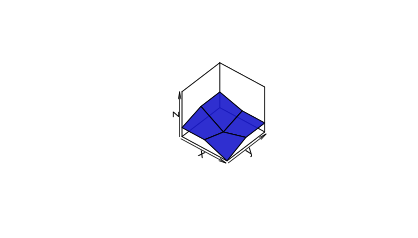
\includegraphics[width=.3\textwidth]{../Bilder/exaktesPotentialSp2.pdf}
	\includegraphics[width=.3\textwidth]{../Bilder/exaktesPotential.pdf}
	\caption{Ein 2-Personenspiel mit exaktem Potential (grau): Spieler 1: rot, Spieler 2: blau}
\end{figure}

Ein exaktes Potential entspricht dann einer gemeinsamen Reliefkarte für beide Spieler, die - im Falle eines exakten Potentials - \glqq scheibenweise\grqq{} bis auf eine additive Konstante mit der eigentlichen Kostenfunktion übereinstimmt. Anders formuliert: Wird dies Strategie eines Spieler festgehalten, so kann der andere Spieler seine Kostenveränderungen bei der Wahl der verschiedenen ihm zur Verfügung stehenden Strategien auch anhand der Potentialfunktion ablesen. 

Geht man nun über zu einem gewichteten Potential, so lesen die beiden Spieler das Potential sozusagen in verschiedenen Einheiten\todo{eigentlich müssen verchiedene Einheiten nicht zwangsläufig proportional zueinander sein - für Längeneinheiten sollte es typischerweise aber stimmen}. Das heißt die Kostenveränderungen eines Spielers sind nur noch proportional zu den Potentialänderungen. Ein skaliertes Potential zeigt jedem Spieler noch an, welche der Kostenveränderungen eher groß und welche klein sind. Ordinale Potentiale zeigen nur noch die Richtung der Kostenveränderung an (\glqq wird teurer\grqq / \glqq wird billiger\grqq / \glqq Kosten bleiben konstant\grqq) und verallgemeinerte ordinale Potentiale zeigen nur noch echte Steigungen korrekt an. Beste-Antwort-Potentiale schließlich zeigen immer die beste Antwort an.


\todo[inline]{Zusammenhänge (evtl. schon nächstes Kapitel?)}

Eine Beobachtung aus \cite{CharExGewPotinWCG}:

\begin{beob}\label{beob:ZshExGewPot}
	Ein Spiel $\Gamma = (I, (X_i)_{i \in I}, (c_i)_{i \in I})$ besitzt genau dann ein gewichtetes Potential (mit Gewichtsvektor $(w_i)_{i \in I}$), wenn $\Gamma' := (I, (X_i)_{i \in I}, (w_i \cdot c_i)_{i \in I})$ ein exaktes Potential besitzt.
\end{beob}

Folgt auch aus einer allgemeineren Beobachtung in \Cref{sec:Morphismen}.

\subsection{Erste Sätze}

Zu einem gegebenen Strategieprofil $x \in X$ sei dessen \emph{Nachbarschaft} die Menge aller durch höchstens eine Abweichung erreichbarer Strategieprofile, d.h. die Menge $\{(\hat{x}_i, x_{-i}) | i \in N, \hat{x}_i \in X_i\}$. Wir nennen $x$ dann ein \emph{lokales Minimum} einer Funktion $f: X \to \IR$, wenn es ein Minimum innerhalb seiner Nachbarschaft ist.

\begin{satz}\label{satz:lokMinNG}
	Sei $\Gamma$ ein Spiel mit einem verallgemeinerten ordinalen Potential $P$. Dann ist jedes lokale Minimum von $P$ ein Nash-Gleichgewicht von $\Gamma$. Ist $P$ sogar ein ordinales Potential, so gilt auch die umgekehrte Richtung.
\end{satz}

\todo[inline]{Diese Sätze hier evtl. nur erwähnen und erst später (nach der Definition von Morphismen) formalisieren (und beweisen)}

Dieser Satz zeigt also, dass man Nash-Gleichgewichte allein durch Betrachten einer Potentialfunktion finden kann. Daraus  folgt direkt die Existenz von Nash-Gleichgewichten in einer Vielzahl von Potentialspielen:

\begin{kor}
	Sei $\Gamma$ ein Spiel mit einem kompakten Strategieraum und einer stetigen verallgemeinerten ordinalen Potentialfunktion. Dann hat $\Gamma$ wenigstens ein Nash-Gleichgewicht.
\end{kor}

Insbesondere also haben endliche Potentialspiele immer ein Nashgleichgewicht. \Cref{satz:lokMinNG} folgt mit Hilfe von \Cref{kor:ExVerbPfadExNG} direkt aus dem folgenden Satz\todo{Streng genommen nicht wirklich, da das Korollar nur für Spiele gilt!?}:

\begin{satz}
	Sei $\Gamma$ ein Spiel mit einem verallgemeinerten ordinalen Potential $P$. Dann ist jeder Verbesserungspfad in $\Gamma$ auch ein Verbesserungspfad bezüglich $P$. Ist $P$ sogar ein ordinales Potential, so gilt auch die umgekehrte Richtung.
\end{satz}

\begin{proof}.
	
	\todo[inline]{Beweis}	
\end{proof}

\todo[inline]{Was kann man über Beste-Antwort-Potentiale sagen (vermtl. Zusammenhang zu Beste-Antwort-Pfade?)}

Für Spiele mit unendlicher Spielermenge erweist es sich als hilfreiche Beobachtung, dass wir Potentiale pfadzusammenhangskomponentenweise definieren können:

\begin{beob}\label{beob:KompWeisePotentiale}
	Sei $\Gamma$ ein beliebiges Spiel und $P: X \to \IR$ eine Funktion. Erfüllt $P$ dann die Bedingung eines exakten/gewichteten/skalierten/ordinalen/verallgemeinerten ordinalen Potentials für jede (maximale) Pfadzusammenhangskomponente, so ist $P$ ein entsprechendes Potential für ganz $\Gamma$.
\end{beob}

\begin{proof}
	Dies folgt direkt aus dem Umstand, dass die definierende Eigenschaft für alle aufgezählten Potentiale immer nur entlang eines Pfades (der Länge $1$) und damit innerhalb einer Zusammenhangskomponente geprüft werden muss.
\end{proof}

\subsection{Charakterisierungen der Potentiale}

\begin{satz}\label{satz:CharExPot}
	Ein Spiel besitzt genau dann ein exaktes Potential, wenn alle 4-Zykel im Strategieraum eine Gesamtänderung von $0$ haben.
\end{satz}

\begin{proof}
	Wir folgen dem Beweis aus \cite[Anhang A]{MonShap}. Dort wird der Satz nur für $N$-Personenspiele gezeigt, mit \Cref{beob:KompWeisePotentiale} überträgt sich dessen Beweis aber direkt auch auf allgemeine Spiele.
	
	Sei zunächst $\gamma \coloneqq (x^0, x^1, x^2, x^3, x^4)$ ein beliebiger 4-Zykel in einem Spiel mit Potential $P$. Dann gilt für die Gesamtänderung:
		\[\delta(\gamma) = \sum_{i=0}^3 c_{i(k)}(x^{k+1}) - c_{i(k)}(x^k) = \sum_{k=0}^{3} P(x^{k+1}) - P(x^k) = P(x^4) - P(x^0) = 0^{}\]
		
	Ist umgekehrt $\Gamma$ ein Spiel, in dem für alle 4-Zykel $\gamma$ gilt $\PfadAend(\gamma) = 0$, $x$ ein beliebiges, aber festes Strategieprofil in $\Gamma$ und $Y_x$ dessen Pfadzusammenhangskomponente. Dann definiere wie folgt eine Funktion $P_x$ auf $Y_x$:
		\[P: Y_x \to \IR: y \mapsto \PfadAend(\gamma), \,\gamma \text{ beliebiger Pfad von } x \text{ nach } y \]
	Damit diese Funktion tatsächlich wohldefiniert ist, muss für je zwei Pfade $\gamma$ und $\gamma'$ von $\hat{x}$ nach $x$ gelten, dass die jeweiligen Gesamtänderungen gleich sind, d.h. $\PfadAend(\gamma) = \PfadAend(\gamma')$. \todo[inline]{weiter (Induktion?)}
	
	Wählen wir nun für jede maximale Pfadzusammenhangskomponente ein einziges $x$ in dieser und definieren wie oben eine Funktion $P_x$, so lassen sich alle diese Funktionen zu einer Funktion $P$ auf ganz $X$ zusammensetzen. Nach Definition erfüllt diese auf jeder Pfadzusammenhangskomponente die Bedingung eines exakten Potentials. Also ist nach \Cref{beob:KompWeisePotentiale} $P$ ein exaktes Potential auf $X$.
\end{proof}

\begin{satz}\label{satz:CharGewPot}
	Ein Spiel besitzt genau dann ein gewichtetes Potential, wenn ... \todo{analoge Bedingung zu exaktem Potential (vgl. \cite[Kapitel 3.2]{CharExGewPotinWCG})}
\end{satz}

\begin{proof}.
	
	\todo[inline]{mit \Cref{beob:ZshExGewPot}?}
\end{proof}

\begin{defn}
	Eine Menge $X$ mit einer strikten Partialordnung $\prec$ (irreflexiv und transitiv) heißt \emph{reell geordnet}\footnote{\citeauthor{CharExOrdPot} bezeichnen solche Mengen in \cite{CharExOrdPot} als \glqq properly ordered\grqq}, wenn es eine strikt monotone Abbildung von $X$ in die reellen Zahlen gib, also $f: X \to \IR$ mit $x \prec x' \implies f(x) < f(x')$.
\end{defn}

Wir definieren nun eine Äquivalenzrelation auf dem Strategieraum:\todo{evtl. schon im Grundlagenkapitel gemeinsam mit Pfadzusammenhangskomponenten?}
	\[x \approx y \colon\iff \text{ es gibt einen nicht-Verschlechterungspfad von $x$ nach $y$ und umgekehrt}\]
Auf dem dadurch erzeugten Raum von Äquivalenzklassen $X/{\approx} \coloneqq \left\lbrace[x] \mid x \in X\right\rbrace$ erhält man eine strikte Partialordnung
	\[[x] \prec [y] \colon\iff x \not\approx y \text{ und es gibt einen nicht-Verschlechterungspfad von $y$ nach $x$}\]

Damit zeigt \citeauthor{CharExOrdPot} in \cite[Theorem 3.1]{CharExOrdPot} folgende Charakterisierung der Existenz von Ordinalen Potentialen:

\begin{satz}\label{satz:CharOrdPot}
	Ein Spiel besitzt genau dann ein ordinales Potential, wenn es keine schwachen Verbesserungszykel enthält und $([X], \prec)$ reell-geordnet ist.
\end{satz}

\begin{proof}
	Sei zunächst $P: X \to \IR$ ein ordinales Potential eines Spiels $\Gamma$. Dann gilt:
	\begin{enumerate}
		\item $\Gamma$ enthält keine schwachen Verbesserungszykel. Denn angenommen $\gamma = (x^0, \dots, x^n)$ wäre ein schwacher Verbesserungszykel in $\Gamma$, so gilt für alle $0 \leq k < n$: $c_{i(k)}(x^{k+1}) \cordleq c_{i(k)}(x^k)$ und für ein solches $k$ sogar $c_{i(k)}(x^{k+1}) \cordle c_{i(k)}(x^k)$. Da ferner $P$ ein ordinales Potential ist, folgt daraus:
			\[P(x^0) \leq P(x^1) \leq \dots \leq P(x^{k+1}) < P(x^k) \leq \dots \leq P(x^n) = P(x^0)\]
		Dies ist jedoch ein Widerspruch. Also kann es keinen solchen Verbesserungszykel geben.
		
		\item $([X], \prec)$ ist reell reell-geordnet. Definiere dazu die Abbildung $f: X/{\approx} \to \IR: [x] \mapsto P(x)$. Diese ist wohldefiniert, denn ist $y \in [x]$, so gibt es also nicht-Verschlechterungspfade von $x$ nach $y$ und umgekehrt. Zusammen bilden dieses einen nicht-Verschlechterungszykel und da es keineschwachen Verbesserungszykel in $\Gamma$ gibt, muss in die diesem Zykel (und damit bereits in den beiden Pfaden) in jedem Schritt Gleichheit gelten. Insbesondere folgt damit $P(x) = P(y)$.
		
		Ferner ist diese Abbildung streng monoton, denn gilt $[x] \prec [y]$, so gibt es einen nicht-Verschlechterungspfad $\gamma$ von $y$ nach $x$, aber keinen in die umgekehrte Richtung. Insbesondere ist also $\overset{\leftarrow}{\gamma}$ kein nicht-Verschlechterungspfad, d.h. $\gamma$ ein schwacher Verbesserungspfad von $y$ nach $x$. Damit folgt analog zum ersten Punkt: $P(x) < P(y)$
	\end{enumerate}

	Ist umgekehrt $([X], \prec)$ reell-geordnet mit Abbildung $f: [X] \to \IR$, so definiere $P: X \to \IR: x \mapsto f([x])$. Dies ist ein ordinales Potential, denn es gilt:
	\begin{enumerate}
		\item Gilt $c_i(x) > c_i(\hat{x}_i, x_{-i})$, so ist $(x, (\hat{x}_i, x_{-i}))$ ein schwacher Verbesserungspfad. Da es in $\Gamma$ keine schwachen Verbesserungszykel gibt, kann es also keinen nicht-Verschlechterungspfad in die andere Richtung geben und es gilt: $[x] \succ [(\hat{x}_i, x_{-i})]$. Daraus wiederum folgt $P(x) = f([x]) > f([(\hat{x}_i, x_{-i})]) = P(\hat{x}_i, x_{-i})$.
		\item Gilt $c_i(x) = c_i(\hat{x}_i, x_{-i})$, so sind sowohl $(x, (\hat{x}_i, x_{-i}))$ als auch $((\hat{x}_i, x_{-i}), x)$ nicht-Verschlechterungspfade, also $[x] = [(\hat{x}_i, x_{-i})]$ und damit $P(x) = f([x]) = f([(\hat{x}_i, x_{-i})]) = P(\hat{x}_i, x_{-i})$. \qedhere
	\end{enumerate}
\end{proof}

\begin{bem}
	Im Gegensatz zur Charakterisierung von exakten Potentialspielen in \Cref{satz:CharExPot} genügt es für die Existenz eines ordinalen Potentials nicht, nur Zykel der Länge 4 zu betrachten. \citeauthor{CharExOrdPot} geben dafür in \cite[Beispiel 3.1]{CharExOrdPot} ein Gegenbeispiel mit zwei Spielern und je drei Strategien an.
\end{bem}

Analog zu \Cref{satz:CharOrdPot} gilt für verallgemeinerte ordinale Potentiale:
\begin{satz}\label{satz:CharVerallOrdPot}
	Ein Spiel besitzt genau dann ein verallgemeinertes ordinales Potential, wenn es keine Verbesserungszykel enthält.
\end{satz}

\begin{proof}
	Sei zunächst $\Gamma$ ein Spiel mit einem verallgemeinerten ordinalen Potential $P$. Angenommen $\gamma = (x^0, \dots, x^n)$ ist ein Verbesserungszykel, d.h. für alle $0 \leq k < n$ gilt $c_{i(k)}(x^{k+1}) \cordle c_{i(k)}(x^k)$. Da $P$ ein verallgemeinertes ordinales Potential ist, folgt daraus $P(x^0) > P(x^1) > \dots > P(x^n) = P(x^0)$, ein Widerspruch. Also kann es keinen Verbesserungszykel geben.
	
	Ist umgekehrt $\Gamma$ ein Spiel, indem es keine Verbesserungszykel gibt. 
	
	\todo[inline]{weiter (geht das überhaupt so allgemein?)}
\end{proof}


\begin{satz}
	Hat ein Spiel die FIP, so besitzt es auch ein verallgemeinertes ordinales Potential.
	
	Umgekehrt besitzt jedes \emph{endliche} Spiel mit einem verallgemeinerten ordinalen Potential auch die FIP.
\end{satz}

\begin{proof}
	\cite{MonShap}/\cite{CongGamesPlayerSpecPayoff} (konstruktiver Beweis)
\end{proof}

\begin{satz}
	Ein Spiel hat genau dann ein Beste Antwort-Potential, wenn es keine beste-Antwort-kompatiblen Kreise enthält und $([X], <)$ properly ordered ist.
\end{satz}

\begin{proof}.
	
	\todo[inline]{aus \cite{BestRespPot}}
\end{proof}